\chapter{Существующие решения}

В этом разделе рассмотрено 3 наиболее распространённых алгоритма асимметричного шифрования, а также приведён результат сравнительного анализа.

\section{Обзор существующих алгоритм асимметричного шифрования}

\subsection{RSA}

Алгоритм RSA был разработан в 1978 году Роном Ривестом, Ади Шамиром и Леонардом Адлеманом, и его название происходит от первых букв фамилий авторов. RSA используется как для шифрования, так и для дешифрования данных. Этот алгоритм применяется для обеспечения конфиденциальности и создания цифровых подписей. Его принцип работы основан на модульной арифметике больших чисел, где создаётся целое число, являющееся произведением двух больших простых чисел. Хотя размер ключа повышает надёжность алгоритма, это также является причиной медленной работы транзакций. Алгоритм RSA состоит из трёх основных шагов: генерация ключа, шифрование и дешифрование~\cite{encrypting}. На рисунке~\ref{fig:rsa} представлена иллюстрация работы алгоритма RSA.

\begin{figure}[H]
	\centering
	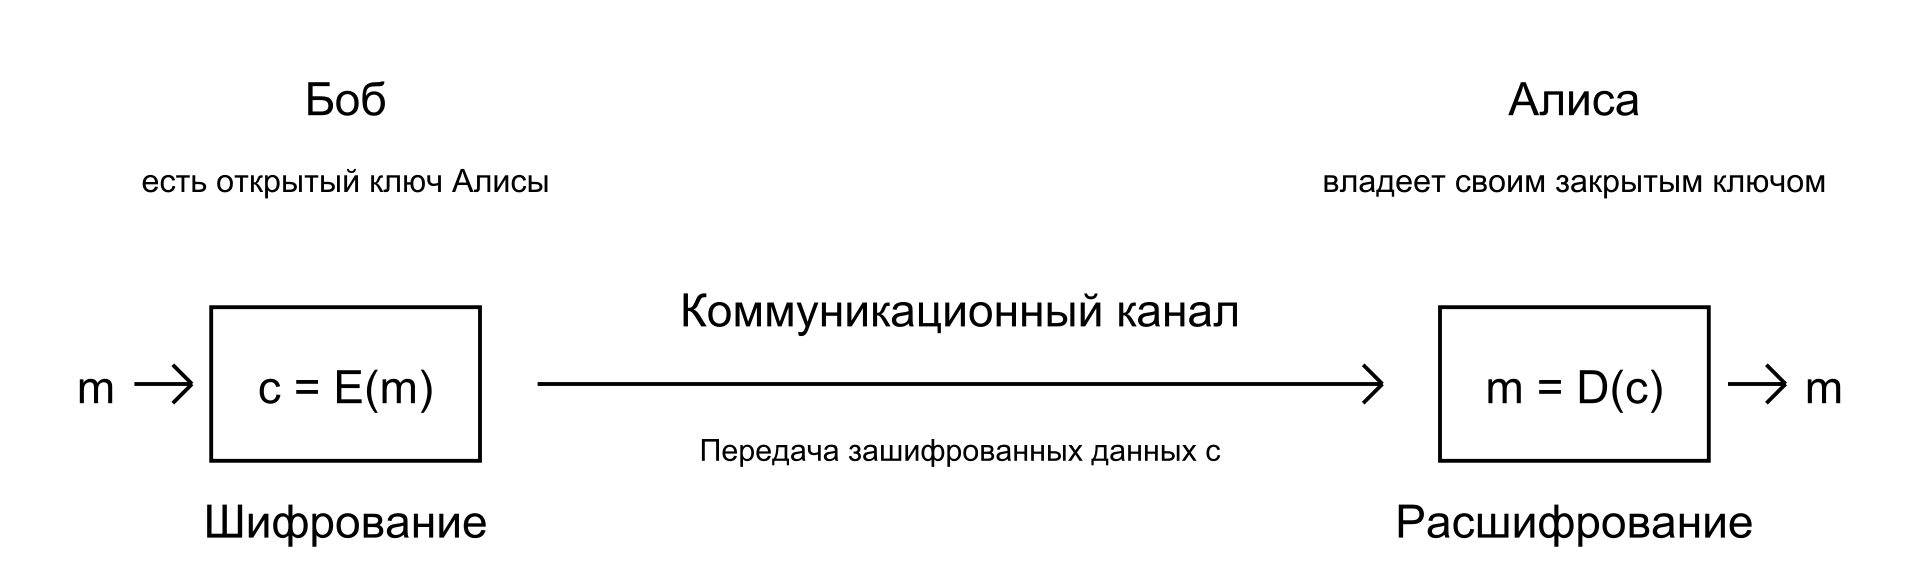
\includegraphics[height=0.2\textheight]{rsa.png}
	\caption{Иллюстрация работы RSA}
	\label{fig:rsa}
\end{figure}

Алгоритм генерации открытого и закрытого ключей состоит из следующих шагов:
\begin{enumerate}
	\item выбор двух больших простых чисел $p$ и $q$;
	\item определение $n$ как результат $p \cdot q$;
	\item выбор случайного $d$ взаимно простого с $(p-1) \cdot (q - 1)$;
	\item определение $e$ такого что $(e \cdot d) \mod ((p-1)\cdot(q-1)) = 1$.
\end{enumerate}

Открытым ключом являются $e$ и $n$, а закрытым -- $d$ и $n$.

Для шифрования данных необходимо:
\begin{enumerate}
	\item разбить текст на блоки, каждый из которых может быть представлен в виде числа $M(i) = 0, 1, 2, ..., n - 1$;
	\item зашифровать блоки по формуле $C(i) = M(i)^e \mod n$.
\end{enumerate}

Расшифрованное сообщение будет получаться по формуле $M(i) = C(i)^d \mod n$. 

\subsection{DSA (алгоритм цифровой подписи)}

Этот алгоритм был утверждён как стандарт цифровой подписи Национальным институтом стандартов и технологий (NIST) в 1991 году. DSA, являющийся алгоритмом с открытым ключом, как и RSA, не использует закрытые ключи для шифрования и открытые — для расшифровки, в отличие от RSA. Для создания цифровой подписи, которая представляет собой 160-битное число, применяется уникальная математическая операция. После того как создаётся хэш сообщения, оно шифруется с использованием закрытого ключа отправителя, что формирует цифровую подпись. При использовании открытого ключа, который связан с закрытым, подтверждается, что сообщение поступило от правильного отправителя~\cite{encrypting}. На рисунке~\ref{fig:dsa} представлена иллюстрация работы алгоритма DSA.

\begin{figure}[H]
	\centering
	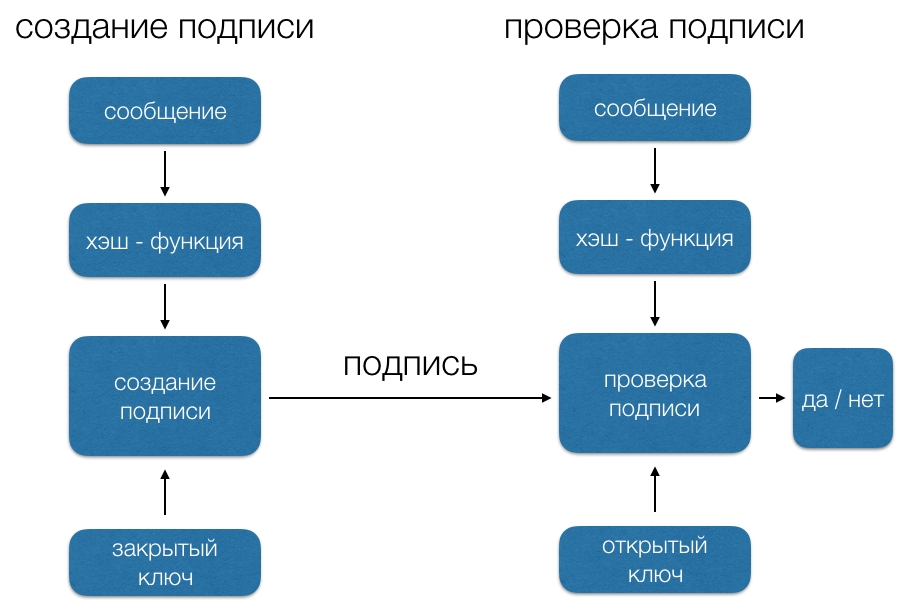
\includegraphics[height=0.4\textheight]{dsa.png}
	\caption{Иллюстрация работы DSA}
	\label{fig:dsa}
\end{figure}

Алгоритм генерации ключа включает в себя следующие шаги:
\begin{enumerate}
	\item выбирается простое число q, такое, что $2^{159} < q < 2^{160}$;
	\item выбирается $t$, такое что $0 \leq t \leq 8$ и выбирается простое число p так, что $2^{511+64t} < p < 2^{512+64t}$, причём $q$ должно делиться на $(p-1)$;
	\item находится производящий элемент $\alpha$ для циклической группы $Z_p$ порядка $q$;
	\item выбирается случайное целое $a$, такое что $1 \leq a \leq q-1$;
	\item вычисляется $y = a^\alpha \mod p$.
\end{enumerate}

Секретным ключом является $a$, а открытым ключом -- $(p, q, \alpha, y)$

Имеется сообщение m. Подпись сообщения секретным ключом выглядит следующим образом:
\begin{enumerate}
	\item выбирается случайное секретное число $k$, $0 < k < q$ (разовый секретный ключ);
	\item вычисляется $r = (\alpha^k \mod p) \mod q$;
	\item вычисляется $k^{-1} \mod q$;
	\item вычисляется $s = k^{-1} (h(m) + \alpha \cdot r) \mod q$ , где h(m) -- значение хэш-функции от сообщения m.
\end{enumerate}

Подписью для сообщения $m$ является пара $(r, s)$.

Имеется открытый ключ $(p, q, \alpha ,y)$, сообщение $m$, подпись сообщения $(r, s)$.
Алгоритм проверки подписи:
\begin{enumerate}
	\item проверить, что $0 < r < q$ и $0 < s < q$. Если это не так, отвергнуть подпись;
	\item вычислить $w = s^{-1} \mod q$ и $h(m)$;
	\item вычислить $u_1 = wh(m) \mod q$ и $u_2 = rw \mod q$;
	\item вычислить $v = (\alpha^{u_1} \cdot y^{u_2} \mod p) \mod q$;
	\item подпись верна, только если $v = r$.
\end{enumerate}

\subsection{ECDSA}

Алгоритм, основанный на сложности вычисления дискретного логарифма в группе точек эллиптической кривой. Эллиптическая кривая в ECDSA -- это линия на плоскости, задаваемая уравнением $y^2 = x^3 + a \cdot x + b$, где a и b -- такие числа, что $4 \cdot a^3 + 27 \cdot b^2 \neq 0$. Например, $Bitcoin$ и $Ethereum$ используют кривую $y^2 = x^3 + 7$ (Рисунок~\ref{fig:ecdsa}).

\begin{figure}[H]
	\centering
	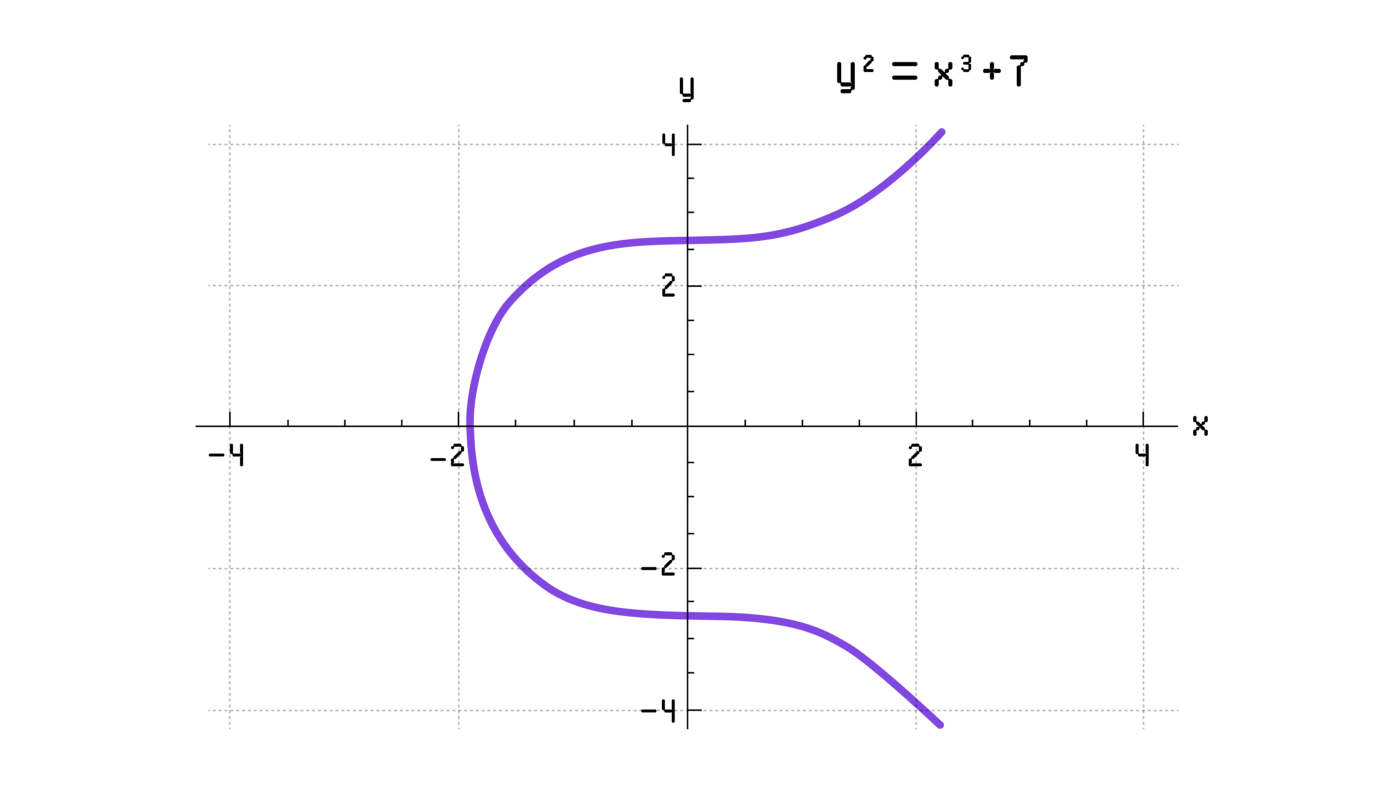
\includegraphics[height=0.4\textheight]{ECDSA.png}
	\caption{Эллиптическая кривая}
	\label{fig:ecdsa}
\end{figure}

Главная особенность эллиптической кривой заключается в том, что её точки можно по особому правилу умножать на целые положительные числа. В результате точка перемещается определенным образом.

Если $G$ -- точка на кривой, а $k$ -- число, то для новой точки $k \cdot G$ есть три варианта расположения:

\begin{enumerate}
	\item $k \cdot G = G$, то есть умножение на $k$ ничего не делает и точка $k \cdot G$ совпадает с $G$. Например, умножение на единицу всегда оставляет точку на месте: $1 \cdot G = G$ для любой $G$. Тут работает аналогия с обычными числами -- умножение на 1 не меняет исходного числа. Так же и с точкой -- её положение на кривой не меняется;
	\item $k \cdot G$ не совпадает с $G$, но при этом все равно лежит на кривой. То есть в результате умножения на q точка как-то скользит вдоль кривой. На рисунке~\ref{fig:dot_moves} приведена схема перемещений конкретной точки $P$ по кривой $y^2 = x^3 + 7$ при умножении на числа от 1 до 7.
	\item Точки $k \cdot G$ не существует. На практике это означает, что в формулах для подсчёта её координат встретилось деление на 0. В этом случае используется специальная терминология: говорят, что $k \cdot G$ -- это бесконечно удалённая точка и пишут $k \cdot G = 0$. 
\end{enumerate}

\begin{figure}[H]
	\centering
	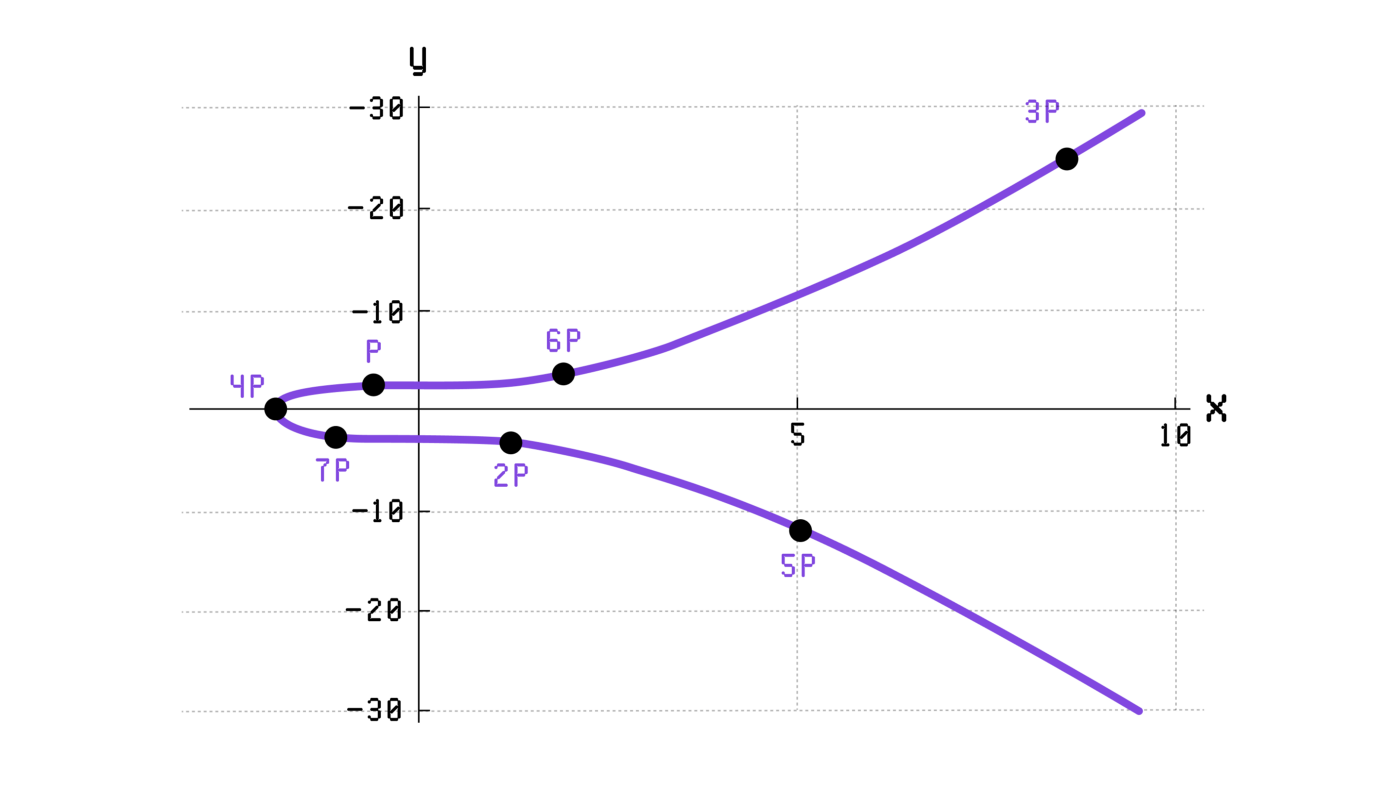
\includegraphics[height=0.4\textheight]{ECDSA_dotmoves.png}
	\caption{Движение точки по эллиптической кривой}
	\label{fig:dot_moves}
\end{figure}

Алгоритм ECDSA предполагает, что в системе заранее выбрано пять параметров, одинаковых для всех пользователей. Два из них относятся к модульной арифметике в ECDSA. Остальные три:

\begin{enumerate}
	\item сама эллиптическая кривая. Чтобы определить кривую, достаточно просто выбрать два числа $a$ и $b$ из её уравнения $y^2 = x^3 + a \cdot x + b$, $4 \cdot a^3 + 27 \cdot b^2 \neq 0$;
	\item простое число $n$;
	\item такая точка $G$ на кривой, что $n$ является порядком $G$. Точка $G$ называется базовой точкой.
\end{enumerate}

Секретный ключ $sk$ выбирается случайным образом от 1 до n-1. В качестве публичного ключа $pk$ берётся точка $pk = sk \cdot G$. 

Здесь в силу вступает ещё одно ключевое свойство операции умножения точки на число. Пусть даны точки $G$ и  $d \cdot G$, где $d$ неизвестно. Тогда оказывается, что найти $d$ — это неразрешимая с вычислительной точки зрения задача. Этот факт называется проблемой дискретного логарифмирования для эллиптических кривых. Отсюда следует, что, зная базовую точку $G$ и публичный ключ $pk$, невозможно найти соответствующий секретный ключ $sk$. На выходе алгоритм выдаёт пару $sk$, $pk$, где $sk$ -- число, а $pk$ -- точка, то есть пара чисел. 

Алгоритм генерации подписи $Sig$ принимает на вход приватный ключ sk и число m — хеш подписываемого сообщения. А на выходе в качестве подписи выдаётся не одно число, а два: $(r, s) = Sig(sk, m)$. Это связано с тем, что внутри самого алгоритма присутствует выбор дополнительного случайного числа $k$, влияющего на вид подписи. Этот случайный параметр нужен для того, чтобы обеспечить секретность ключу $sk$. Если подпись полностью определятся лишь входными параметрами $sk$ и $m$, то секретный ключ $sk$ может быть вычислен на основе всего лишь двух оставленных с его помощью подписей. Наличие случайного параметра приводит к тому, что на одних и тех же входных значениях алгоритм $Sig$ может выдавать разный результат. Поэтому, чтобы подпись можно было проверить, необходимо поделиться некоторой информацией о параметре $k$. Первая компонента подписи $r$ как раз содержит в себе эту информацию. Число $r$ полностью определяется числом $k$, при его подсчёте $sk$ и $m$ не используются. В то же время в вычислениях числа $s$ участвуют уже все три параметра $k$, $sk$ и $m$.

Алгоритм проверки подписи $Ver$ принимает на вход публичный ключ $pk$, хеш сообщения $m$ и подпись $(r, s)$. На основе подписи и хеша этот алгоритм находит два числа $u_1$ и $u_2$. Далее рассматриваются две точки на эллиптической кривой: $u_1 \cdot G$ и $u_2 \cdot pk$ ($pk$ — точка, значит, $u_2 \cdot pk$ — тоже точка). Если подпись $s$ была действительно посчитана с помощью ключа $sk$, соответствующего ключу $pk$, и сообщение действительно не менялось с момента создания подписи, то точки $u_1 \cdot G$ и $u_2 \cdot pk$ будут находится относительно друг друга в некотором специальном положении. Алгоритм $Ver$ смотрит, так это или нет. Если расположение точек относительно друг друга и правда такое, какое должно быть, то подпись считается корректной, и $Ver$ возвращает 1 (TRUE). В противном случае возвращается 0 (FALSE).~\cite{ECDSA}

\section{Критерии сравнения алгоритмов}

В таблице~\ref{tbl:criterions} приведены критерии, которые будут использоваться для сравнительного анализа существующих методов асимметричного шифрования.

\begin{table}[H]
	\begin{center}
		\begin{threeparttable}
			\captionsetup{justification=raggedright,singlelinecheck=off}
			\caption{\label{tbl:criterions} Критерии сравнения алгоритмов асимметричного шифрования}
			\begin{tabular}{|p{4cm}|p{10cm}|}
				\hline
				Критерий & Описание \\ \hline
				Безопасность & Сложность криптоанализа: Оценка того, насколько устойчив алгоритм к попыткам взлома, включая анализ стойкости против атак, таких как атаки с использованием вычислительных мощностей, и атаки на основе математических принципов.
				
				Размер ключа: Чем больше длина ключа, тем сложнее взломать алгоритм, но это также может повлиять на производительность. \\ \hline
				Производительность & Скорость шифрования/дешифрования: Важный фактор для практического применения, особенно в системах с ограниченными ресурсами (например, мобильных устройствах или IoT).
				
				Эффективность вычислений: Требования к вычислительным мощностям (процессору и памяти) для выполнения операций шифрования и дешифрования. \\ \hline
				
			\end{tabular}
		\end{threeparttable}
	\end{center}
\end{table}
	
\section{Сравнительный анализ алгоритмов}

В таблице~\ref{tbl:results} представлены результаты сравнительного анализа. Цифра в ячейке обозначает преимущество перед другими алгоритмами: 3 -- алгоритм наиболее эффективен по данному критерию, 1 -- алгоритм наименее эффективен по данному критерию (среди представленных).

\begin{table}[H]
	\begin{center}
		\begin{threeparttable}
			\captionsetup{justification=raggedright,singlelinecheck=off}
			\caption{\label{tbl:results} Результаты сравнительного анализа}
			\begin{tabular}{|p{5cm}|p{2cm}|p{2cm}|p{2cm}|}
				\hline
				Критерий & RSA & DSA & ECDSA \\ \hline
				Безопасность (Сложность криптоанализа) & 1 & 2 & 3 \\ \hline 
				Безопасность (Размер ключа) & 2 & 1 & 3 \\ \hline
				Производительность (Скорость шифрования/дешифрования) & 2 & 3 & 1 \\ \hline
				Производительность (Эффективность вычислений) & 1 & 3 & 2 \\ \hline 
			\end{tabular}
		\end{threeparttable}
	\end{center}
\end{table}
